%!TEX root = ../../main.tex

\chapter{Architektur}

\section{Anforderungen}

Im Folgenden werden anhand der aufgelisteten internen und externen Stakeholder die funktionalen und nicht-funktionalen Anforderungen aufgeführt.

Interne Stakeholder

\begin{itemize}
  \item Entwickler
  \item Betreuer
  \item Systemadministrator
\end{itemize}

Externe Stakeholder
\begin{itemize}
  \item Nutzer
\end{itemize}

\subsection{Funktionale Anforderungen}
\begin{itemize}
  \item Client Kommunikation: 
    Als Nutzer und Entwickler möchte ich mich über WebSockets mit dem System verbinden können, wobei ich zwischen einem CLI- und einem WASM-Client entscheiden möchte, damit ich meine präferierte Umgebung verwenden kann. Ich möchte Nachrichten in Echtzeit senden und empfangen, Räumen beitreten und verlassen, sowie meinen Anzeigenamen ändern können. Darüber hinaus soll es möglich sein, vergangene Nachrichten laden zu können, damit ich den gesamten Chatverlauf einsehen kann.
  \item Loadbalancer: Als Nutzer und Systemadministrator möchte ich, dass ein Loadbalancer die WebSocket Verbindungen gleichmäßig auf die vorhandenen Backends verteilt, damit eine optimale Performance erreicht werden kann. Wenn ein Backend ausfällt, sollen die bestehenden Verbindungen nahtlos vom Loadbalancer zu anderen Backends umgeleitet werden, sodass ich beim Benutzen keine Unterbrechung bemerke.
  \item Backend Services: Als Entwickler möchte ich, dass die Client Verbindungen vom Backend verwaltet werden und Nutzer spezifische Buffer verwendet werden, um Nachrichten effizient und zuverlässig verarbeiten zu können. Nachrichten sollen über ein Publish/Subscribe-System verteilt werden, damit alle Backendinstanzen synchron sind und in einer Datenbank gespeichert werden, um Chatverläufe abrufen zu können. Das System soll Pub/Sub-Mechanismen als Cluster unterstützen, damit es Skalierbar und Ausfallsicher ist.
\end{itemize}
\subsection{Nichtfunktionale Anforderungen}
\begin{itemize}
  \item Hohe Verfügbarkeit: Als Nutzer, Systemadministrator und Betreuer möchte ich, dass das System weiterhin funktioniert, auch wenn ein Backend ausfällt, ohne das der Nutzer eine Unterbrechung mitbekommt. Nach dem Ausfall eines Backends soll die Verbindung automatish von einem anderen Backend übernommen werden ohne das Nachrichten verloren gehen.
  \item Zuverlässigkeit: Als Nutzer und Systemadministrator möchte ich, dass Nachrichten zugestellt werden, solange die Datenbank und mindestens ein Backend verfügbar sind, so dass Nachrichten nicht verloren gehen, auch wenn Teile des Systems ausfallen. Die Konsistenz der Daten soll durch eine Datenbank sichergestellt werden, sodass keine Nachrichten des Chatverlaufs fehlen und dieser damit eindeutig und zuverlässig ist.
  \item Skalierbarkeit: Als Entwickler und Betreuer möchte ich, dass das System horizontal skalierbar ist, damit es auch unter hoher Last performant bleibt. Es sollen mehrere verteilte Pub/Sub-Instanzen und Backends verwendet werden.
\end{itemize}

\section{Architekturentscheidungen}
% Warum Redis?
% Start mit einem Container
% Redis Cluster
% Redis Redundancy
% Warum PostgreSQL-Datenbank?
% Warum Nginx? Warum diese Strategie (least connections)?

\subsection{Rust}
Als Programmiersprache wird Rust genutzt.
Da Rust so vielseitig einsetzbar ist wird diese für die Clients als auch für das Backend verwendet.
Dabei wird im Backend die Rust-Library \textit{tokio} genutzt, um Asynchrone Aufgaben zu verwalten.
Im \ac{WASM}-Client wird die Rust-Library \textit{wasm-bindgen} genutzt, um WebAssembly zu nutzen.
Im \ac{CLI}-Client wird die Rust-Library \textit{ratatui} genutzt, um die Kommandozeile als User Interface zu nutzen.
Die Programmiersprache wurde aus bestehendem Eigeninteresse in diesem Projekt verwendet und da es die beliebteste Programmiersprache ist, wie in einer Umfrage von Stackoverflow herausgefunden wurde.\footnote{\glcite{stackoverflow_survey:2025}}

\subsection{Redis}
Redis ist eine in-memory Datenbank, die eine einfache und schnell zu verwendende, leistungsfähige, skalierbare und zuverlässige Datenbank ist.
Allerdings ist der Hauptnutzen für das System in dieser Arbeit die Publish und Subscribe Funktionalität.
Das Setup eines Redis Containers ist sehr einfach und benötigt wenig Konfiguration, dadurch eignet sich Redis als Kommunikationsschnittstelle unter den Backendinstanzen.

\subsection{Loadbalancer}
Als Loadbalancer wird \textit{Nginx} genutzt. 
Nginx bietet nicht nur Stabilität und bewährte Performance, sondern ermöglicht auch flexible Strategien 
zur Lastverteilung.  
In diesem Projekt wird die Strategie \textit{Least Connections} verwendet. Dabei werden neue Verbindungen 
an den Server mit den aktuell wenigsten aktiven Verbindungen weitergeleitet.  
Dies führt zu einer gleichmäßigeren Auslastung der Backend-Instanzen, insbesondere in Szenarien mit 
langen Verbindungen, wie sie bei WebSocket-Kommunikation üblich sind.

\subsection{PostgreSQL-Datenbank}
Für die persistente Datenspeicherung wird eine \textit{PostgreSQL}-Datenbank eingesetzt.  
PostgreSQL wurde gewählt, da sie ein stabiles, weit verbreitetes und leistungsfähiges relationales Datenbanksystem ist. 
Die Datenbank PostgreSQL wurde auch ausgewählt, da die Entwickler dieses Projekts bereits mit PostgreSQL gearbeitet haben.
Die Trennung zwischen Redis (für flüchtige, schnelle Daten) und PostgreSQL (für persistente Daten) 
ermöglicht eine klare Architektur, bei der beide Systeme ihre jeweiligen Stärken optimal ausspielen können.
Jede andere relationale SQL-Datenbank wie MySQL oder MariaDB hätte im Rahmen dieses Projekts auch ausgereicht.

\section{Systemkomponenten}
Das System besteht aus fünf Komponenten: \textit{Client}, \textit{Backend}, \textit{Redis-Cluster}, \textit{Loadbalancer} und \textit{Datenbank}.

\begin{description}[style=nextline]
    \item [Client] Es gibt zwei verschiedene Arten von Clients: 
        \begin{itemize} 
            \item \textit{\ac{CLI}} 
            \item \textit{\ac{WASM}}
        \end{itemize}
        Beide Clients verbinden sich mit dem Loadbalancer, dieser leitet auf eine Backendkomponente weiter, um Nachrichten zu senden und zu empfangen.

    \item [Backend] Die Backendkomponente ist ein in Rust geschriebener Websocket-Server.
        Diese verwaltet die Nachrichten und kommuniziert über das Redis-Cluster mit den anderen Backendinstanzen.
        Zu dem persistiert diese die Nachrichten und Informationen über den Nutzer in einer Datenbank.
        Es werden zur Ausfallsicherheit drei Instanzen aufgesetzt.

    \item [Redis-Cluster] Das Redis-Cluster ist die Kernkomponente für die Synchronisation der Nachrichten und stellt die Kommunikation unter den Backendinstanzen her.
        Dafür wird die Publish und Subscribe Funktion von Redis genutzt.
        Jeder Chatraum wird als Channel in Redis abgebildet.
        Jede Nachricht des Clients wird auf den jeweiligen Channel in Redis gepublished.
        Um eine Nachricht zu erhalten erstellt das Backend für jeden Client einen Subscriber auf dem entsprechenden Channel.
        Das Redis-Cluster besteht aus sechs Redis-Nodes, drei davon sind Master-Nodes und die restlichen drei sind zu den Master-Nodes die jeweiligen Replicas.

    \item [Loadbalancer] Der Loadbalancer ist eine Komponente, die die Verbindungen zwischen den Clients und den Backends verteilt.
        Als Loadbalancer wird Nginx genutzt, da dieser einer der renomiertesten in dieser Technologie ist.
        Als Strategie zur Aufteilung auf die Backendinstanzen wird nach dem Verfahren der wenigsten Verbindungen vorgegangen.

    \item [Datenbank] Die Datenbank ist eine PostgreSQL-Datenbank, die die Nachrichten und Informationen der Nutzer speichert.
        Die Backendinstanzen verbinden sich mit der Datenbank, um die Nachrichten zu laden und zu speichern.
        Zusätzliche werden die Nutzerinformationen und in welchem Chatraum diese sich befinden gespeichert.
        Die Datenbank ist keine Systemkritischen Komponente und sorgt im Falle eines Ausfalls nur für eine Funktionseinschränkung.
\end{description}


% Architekturdiagramm hier einfügen oder drüber
\begin{figure}[H]
    \centering
    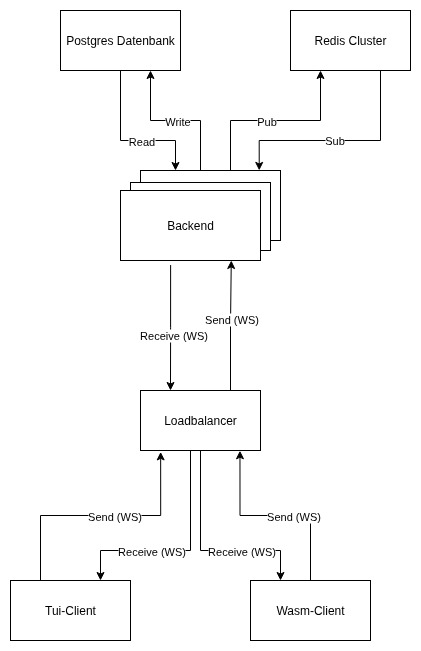
\includegraphics[width=0.8\textwidth]{images/architecture.png}
    \caption{Architekturdiagramm}
    \label{fig:architecture}
\end{figure}
